\chapter{Literature Review}

\section{Machine learning of morphology: sub-problems and related problems}

Within the realm of machine understanding of morphology, there are many sub-problems and related problems. The most basic areas of research involve predicting the morphology of words in isolation - transforming a word into a specific morphological form, or the inverse, tagging a form with its morphological categories. Typically, this has been done with words in regular grammatical paradigms, such as number and case marking on nouns, or tense, aspect, mood, and/or argument agreement patterns on verbs. 

\subsection{Core supervised learning problems}

Some of the earliest work in computational morphology involves making specific morphological transformations. That is, given a particular form of a lexeme (often, but not necessarily, a citation form), predicting another form. An example would be learning to transform English verbs from present to past tense, e.g., \textit{show} $\rightarrow$ \textit{showed}, \textit{see} $\rightarrow$ \textit{saw}, etc. \parencite{Dreyer2008}.

The natural extension of this is aiming to be able to predict any inflected form given one specific form of a lexeme and an arbitrary set of morphological categories. For instance, given a lexeme \textit{see} and the categories \texttt{3rd person singular, simple present}, generating the correct form \textit{sees}. Generally speaking, a citation form has been used as input \parencite{Durrett2013} \parencite{Faruqui2015} \parencite{Cotterell2017}. The related "reinflection" problem involves being given any inflected form as input, and transforming it into any other \parencite{Cotterell2016}.

A further extension of the morphology generation problem is the generation of complete inflection tables. The exact nature of this problem depends on the type of training and test data used. If a model is only trained on a sparse, random sampling of forms for each lexeme, then a task may consist of filling out the rest of an inflection table for those lexemes. For instance, a model may be given the forms \textit{sees} and \textit{seeing} among its training data, and be required to fill out the remaining forms of that paradigm, including \textit{see} and \textit{saw}. 

If a model is instead trained using entire inflection tables, e.g., all forms of the verb \textit{see}, then test data must consist of new lexemes. Another dimension along which paradigm completion tasks differ is whether only a single citation form is provided as a prompt, or whether any form or even multiple forms may be provided as a prompt for producing a single table \parencite{Hulden2014} \parencite{Ahlberg2015} \parencite{Cotterell2017}.

\subsection{Inflection types}

Overall, a diverse set of inflection shapes have been worked with in the most recent efforts of this subfield. Since 2016, the Special Interest Group on Computational Morphology and Phonology (SIGMORPHON), a research collective focused on computational morphology and related problems, has fielded "shared tasks" in which several research teams globally are given training data and a task definition, and attempt to create models which are subsequently compared. The SIGMORPHON shared task 2018 included training data from 103 typologically diverse languages, and paradigms using suffixing, prefixing, infixing, reduplication, and non-concatenative morphology. 

However, all SIGMORPHON work has been with well-defined, tabular paradigms of grammatical inflection of fairly moderate size ($\leq 200$ forms) \parencite{Cotterell2018b}. Other types of morphology such as derivational morphology and cliticization, which have the potential to greatly expand the number of possible forms and in a less organized fashion, have been less well explored. What \cite{Mattissen2004} calls "compositionally polysynthetic" languages, those which make extensive use of more expansive types of word building including incorporation and productive derivational morphology, are ripe for future work \parencite{Cotterell2016}. Such languages include Chukchi, Cherokee, Ainu, Nahuatl, and others \parencite{Mattissen2004}.

The chief challenges with approaching these less paradigmatic types of inflection are data procurement and structuring. For grammatical inflection paradigms, the set of potential forms is simply combinatorial from the set of grammatical categories, and can be specifically enumerated. Concretely, the vast majority of grammatical paradigm data used in SIGMORPHON comes from Wiktionary, a free and collaborative online multilingual dictionary which provides full or partial tables of grammatical inflection along with lexeme definitions; these tables define the space of inflected forms for the task. In contrast, with derivational morphology, noun incorporation, and other less paradigmatic types of inflection, the possibility space is considerably less well-defined. How can a model know a priori that \textit{likeable} is a valid word of English but \textit{hateable} is not, or that the opposite of \textit{accessible} is \textit{inaccessible} and not \textit{unaccessable}? There are no tables for the set of, e.g., derivational forms that a lexeme may take on, since it is constrained by semantics and idiosyncratic usage, and there is considerably more variability among lexemes of the same category (say, verbs) in which derivational categories they may take on than which grammatical categories. Consequently, labeled data is much harder to come by, and it is harder to demonstrate that a dataset of derivational forms is truly exhaustive.

\subsection{Related problems}

Within only the last two or so years, there has been work on predicting morphology in context. In the 2018 and 2019 SIGMORPHON shared tasks, to which several teams of researchers submitted solutions, a sub-task was dedicated to cloze challenges, a type of test in which one word in a sentence, given in citation form, was to be inflected based on context \parencite{Cotterell2018b} \parencite{McCarthy2019}. This work is essentially a synthesis of morphology generation and morphosyntactic modeling.

Since 2017, there has been some work done on learning curves for computational morphology. The datasets published for SIGMORPHON 2017 and 2018 include partitions into low ($\sim$100 forms), medium ($\sim$1000 forms), and high ($\sim$10,000 forms) data training sets for the express purpose of assessing the learning curve of different models. Evidence suggests that learning curve varies by model type; LSTM neural models, a type of model generally considered to be state of the art, despite being the most successful models with high-data training sets, often fare worse than more baseline string transduction models with low data training sets \parencite{Cotterell2017} \parencite{Cotterell2018b}. Improving performance with small training sets is of interest, as much of the applicability of computational morphology models is to languages which don't already have high-quality technical tools or datasets. 

The most recent new challenge that SIGMORPHON has tried to address is that of transfer learning of morphology, in the shared task earlier this year. Given a state of the art model trained on a language with a high volume of training data, teams were asked to alter it into a model that would perform well on a new language, given a smaller amount of training data for that language. 80\% of the pairs of languages were closely related, while 20\% were distantly or not at all related. Gains of transfer learning models between closely related languages generally performed better than transfer learning models between more distant languages \parencite{McCarthy2019}.

\section{Non-neural approaches}

\subsection{Vector embedding}

A technique that has found success in a variety of computational linguistics tasks is that of representing words in relatively low-dimensional vector spaces. That is, words are represented as a vector, a series of numbers of fixed length; the length of the vector is typically much smaller than the number of total known words. This has the intention of capturing semantic and syntactic content in a principled way - similarity between the number of two words are expected to signify actual similarity in their meaning, and regular linear transformations between vectors should roughly correspond to specific semantic or grammatical changes. These vector representations can be generated via various unsupervised learning methods \parencite{Bilmes2003} \parencite{Alexandrescu2006}.

Regularities in the relative location of semantically related words have been exploited for semantic analysis tasks \parencite{Alexandrescu2006}. Similarly, morphological changes may appear as spatial transformations in vector space, and work has been done on discovering morphological relationships between in-vocabulary words based on their relative spatial locations \parencite{Mikolov2013} \parencite{Soricut2015} \parencite{DosSantos2014}. Figure 2.1 illustrates this idea in a slightly simplified way: once a vector embedding model has been trained on English, it can be discovered that semantic transformations (male to female) and grammatical transformations (singular to plural) roughly correspond to regular spatial translations in vector space.

Vector embedding has the limitation that it cannot extend to words for which a vector representation has not been trained, and so it cannot directly provide understanding of the many OOV forms encountered in test data of highly inflected languages \parencite{Soricut2015} \parencite{Cotterell2019}. However, it can be a means to discover relationships between words in an unsupervised manner, which may support labeling tasks in support of computational morphology and other tasks.

\begin{figure}[t]
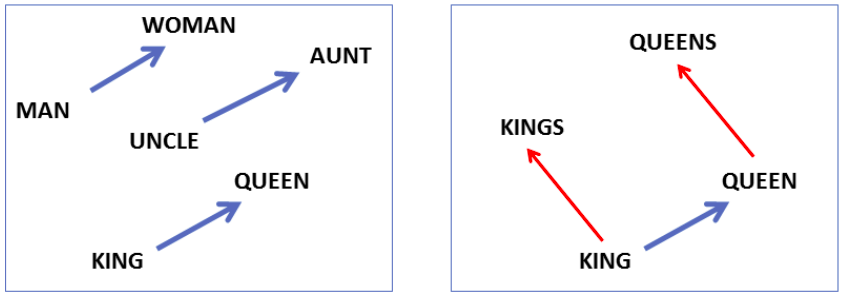
\includegraphics[width=12cm]{images/semantic_transform.png}
\centering
\caption{Regular spatial transformations encode semantic or grammatical content \parencite{Mikolov2013}}
\end{figure}

\subsection{String transduction}

Earlier work specifically focused on the problem of morphology prediction made use of iteratively improving methods of string transduction - in essence, pattern matching on the written representations of words \parencite{Durrett2013} \parencite{Hulden2014} \parencite{Nicolai2015} \parencite{Ahlberg2015}. Typical steps of string transduction methods include character alignment (depicted in Figure 2.2), identification of characters that are inserted or deleted based on grammatical form, and generalization of lexemes which are inflected by the same sets of insertions or deletions (depicted in Figure 2.3). 

\begin{figure}[t]
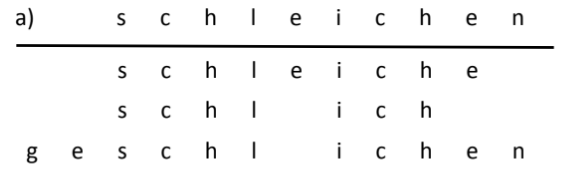
\includegraphics[width=12cm]{images/Nicolai2015_schleichen.png}
\centering
\caption{Character alignment for various forms of the German verb \textit{schleichen} \parencite{Nicolai2015}.}
\end{figure}

\begin{figure}[t]
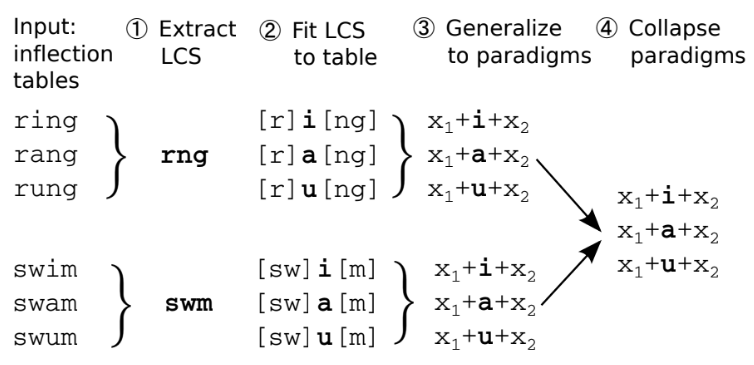
\includegraphics[width=12cm]{images/Hulden2014_diagram.png}
\centering
\caption{Conceptual depiction of a typical example of a string transduction method of morphology learning \parencite{Hulden2014}.}
\end{figure}

A crucial limitation of string transduction methods are their general assumption that most lexemes have exactly the same set of characterwise transformations as a large group of other lexemes, and that a manageably small number of such inflection classes exist. There are paradigms with such a limited set of inflection classes, such as Spanish \textit{-ar}, \textit{-er}, and \textit{-ir} verbs. However, when multiple morpholonological processes are at play, individual lexemes may be nearly unique in their exact set of transformations.

For example, Finnish noun declension has processes of vowel harmony, consonant gradation, and vowel alternation and lengthening operating to produce final inflected forms \parencite{Ranta2008}. As an illustration, consider the Finnish nouns \textit{puku} "suit" and \textit{kenkä} "shoe", which have the inessive singular forms \textit{puvussa} "in the suit" and \textit{kengässä} "in the shoe", respectively. In both forms, the letter \textit{k} is transformed via consonant gradation, but the letter it becomes depends on the surrounding letters. The final vowel of the forms may be \textit{a} or \textit{ä}, depending on vowel harmony. In other inflected forms, the final vowel of the words may be doubled \parencite{Wiktionary}. A model that naively seeks to match these words with other words using the same set of character transformations across the paradigm may need to assign nearly every word to its own category, failing to generalize the patterns at work.

The poorer performance of string transduction relative to neural models has led to a move of the field away from string transduction since about 2016 \parencite{Cotterell2018b}.

\section{LSTM and other neural approaches}

Since 2016, almost all work on paradigm completion has made use of long short-term memory (LSTM) or related gated recurrent network (GRU) models \parencite{Faruqui2015} \parencite{Cotterell2016} \parencite{Cotterell2017} \parencite{Cotterell2018b} \parencite{McCarthy2019}. An LSTM network is a variation on a recurrent neural network (RNN), a variant of neural network \parencite{Hochreiter1997}.

Neural networks are a type of function approximation model inspired by the connection of neurons in animal brains. They have come to be implemented in a variety of forms, and underlie state of the art machine learning models in a variety of applications. The common feature of neural models is repeated matrix multiplication followed by the application of a non-linear "activation" function. Figure 2.4 illustrates a simple feed-forward network, in which a vector of three inputs is multiplied by some $3 \times 4$ matrix and activated to produce a vector of four intermediate values, which are again multiplied by some $4 \times 2$ matrix and activated to produce a vector of two outputs.

An RNN is a type of neural network that operates over sequences of inputs, typically with unknown length. Figure 2.5 illustrates the general structure: each input is represented by a vector, which is multiplied by a vector $U$ to modify state, and the modified state is then multiplied by a vector $W$ to produce an output vector and a matrix $V$ to produce the next state. An LSTM network utilizes a specific means of using the inputs to modify state, represented by Figure 2.6, which includes the ability to modify the rate at which information is forgotten. LSTMs are intended to solve the forgetfulness of earlier RNN types, which tend to be unable to recall information from more than a few iterations prior \parencite{Hochreiter1997}.

\begin{figure}[t]
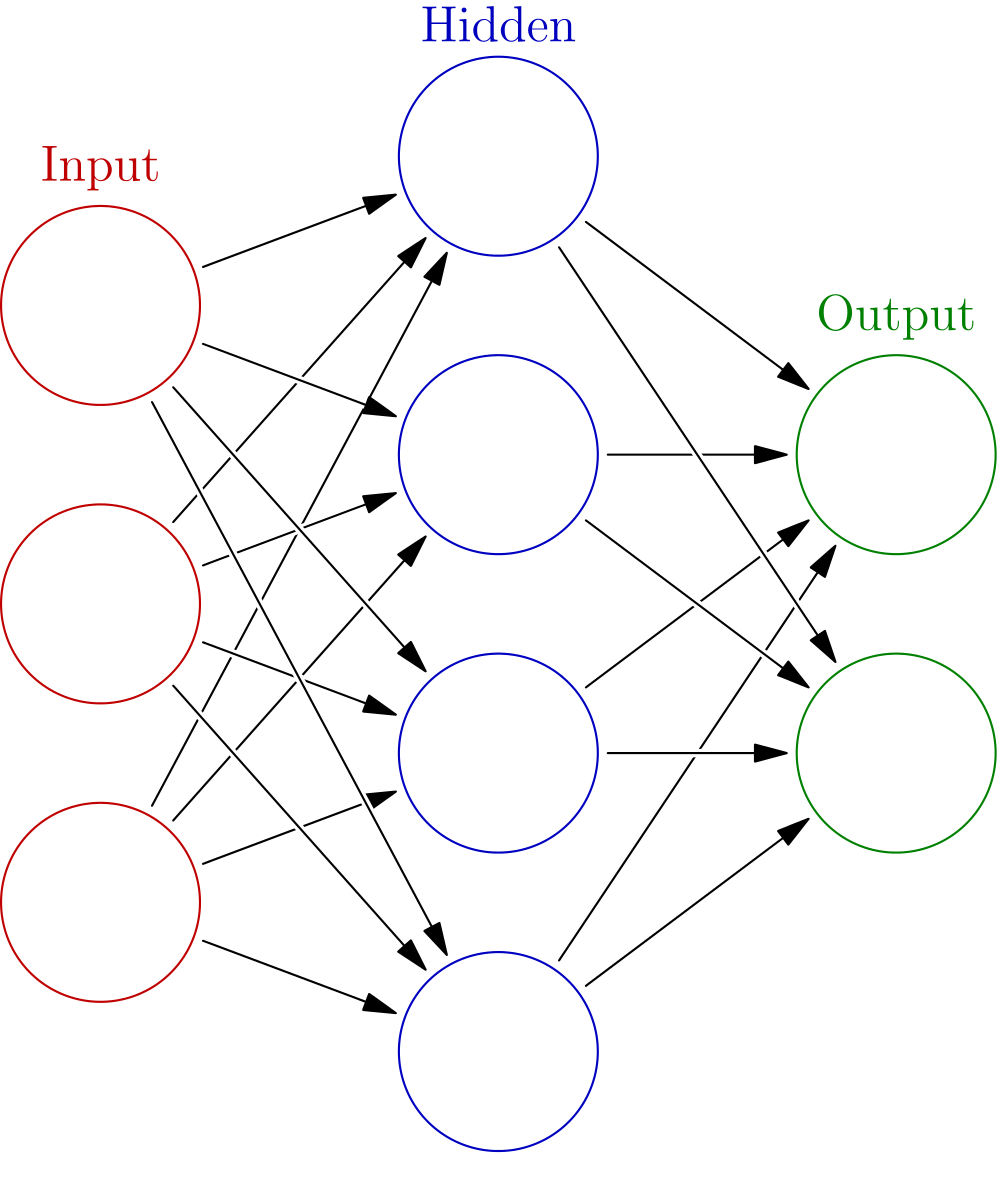
\includegraphics[width=6cm]{images/1000px-Colored_neural_network.png}
\centering
\caption{The structure of a feed-forward neural network with three inputs, four hidden cells, and two outputs. (commons.wikimedia.org/wiki/File:Colored\_neural\_network.svg)}
\end{figure}

\begin{figure}[t]
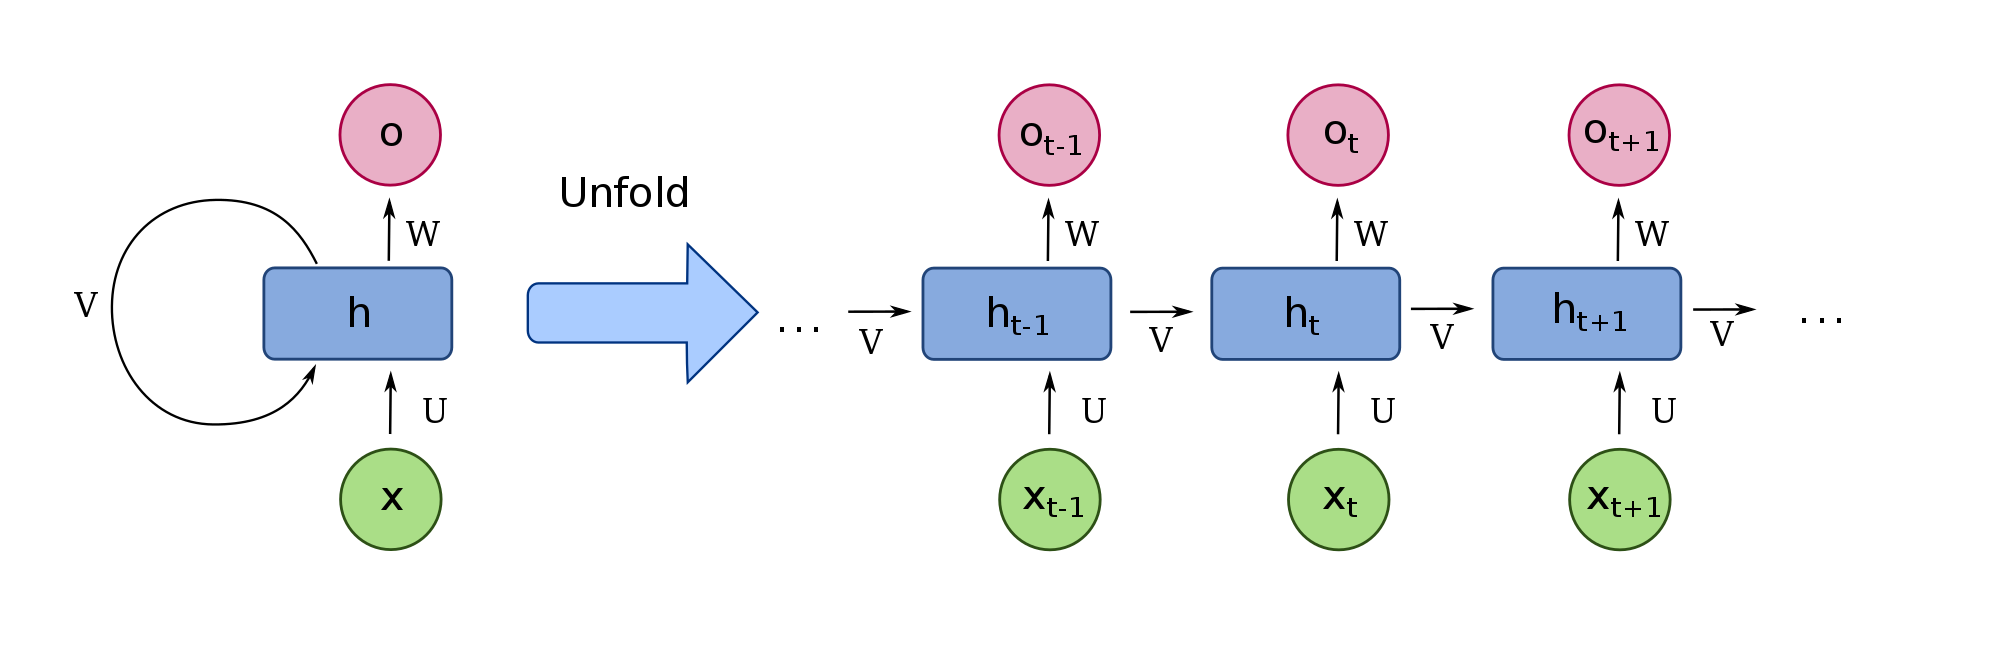
\includegraphics[width=12cm]{images/RNN.png}
\centering
\caption{The generalized structure of a recurrent neural network. (commons.wikimedia.org/wiki/File:Recurrent\_neural\_network\_unfold.svg)}
\end{figure}

\begin{figure}[t]
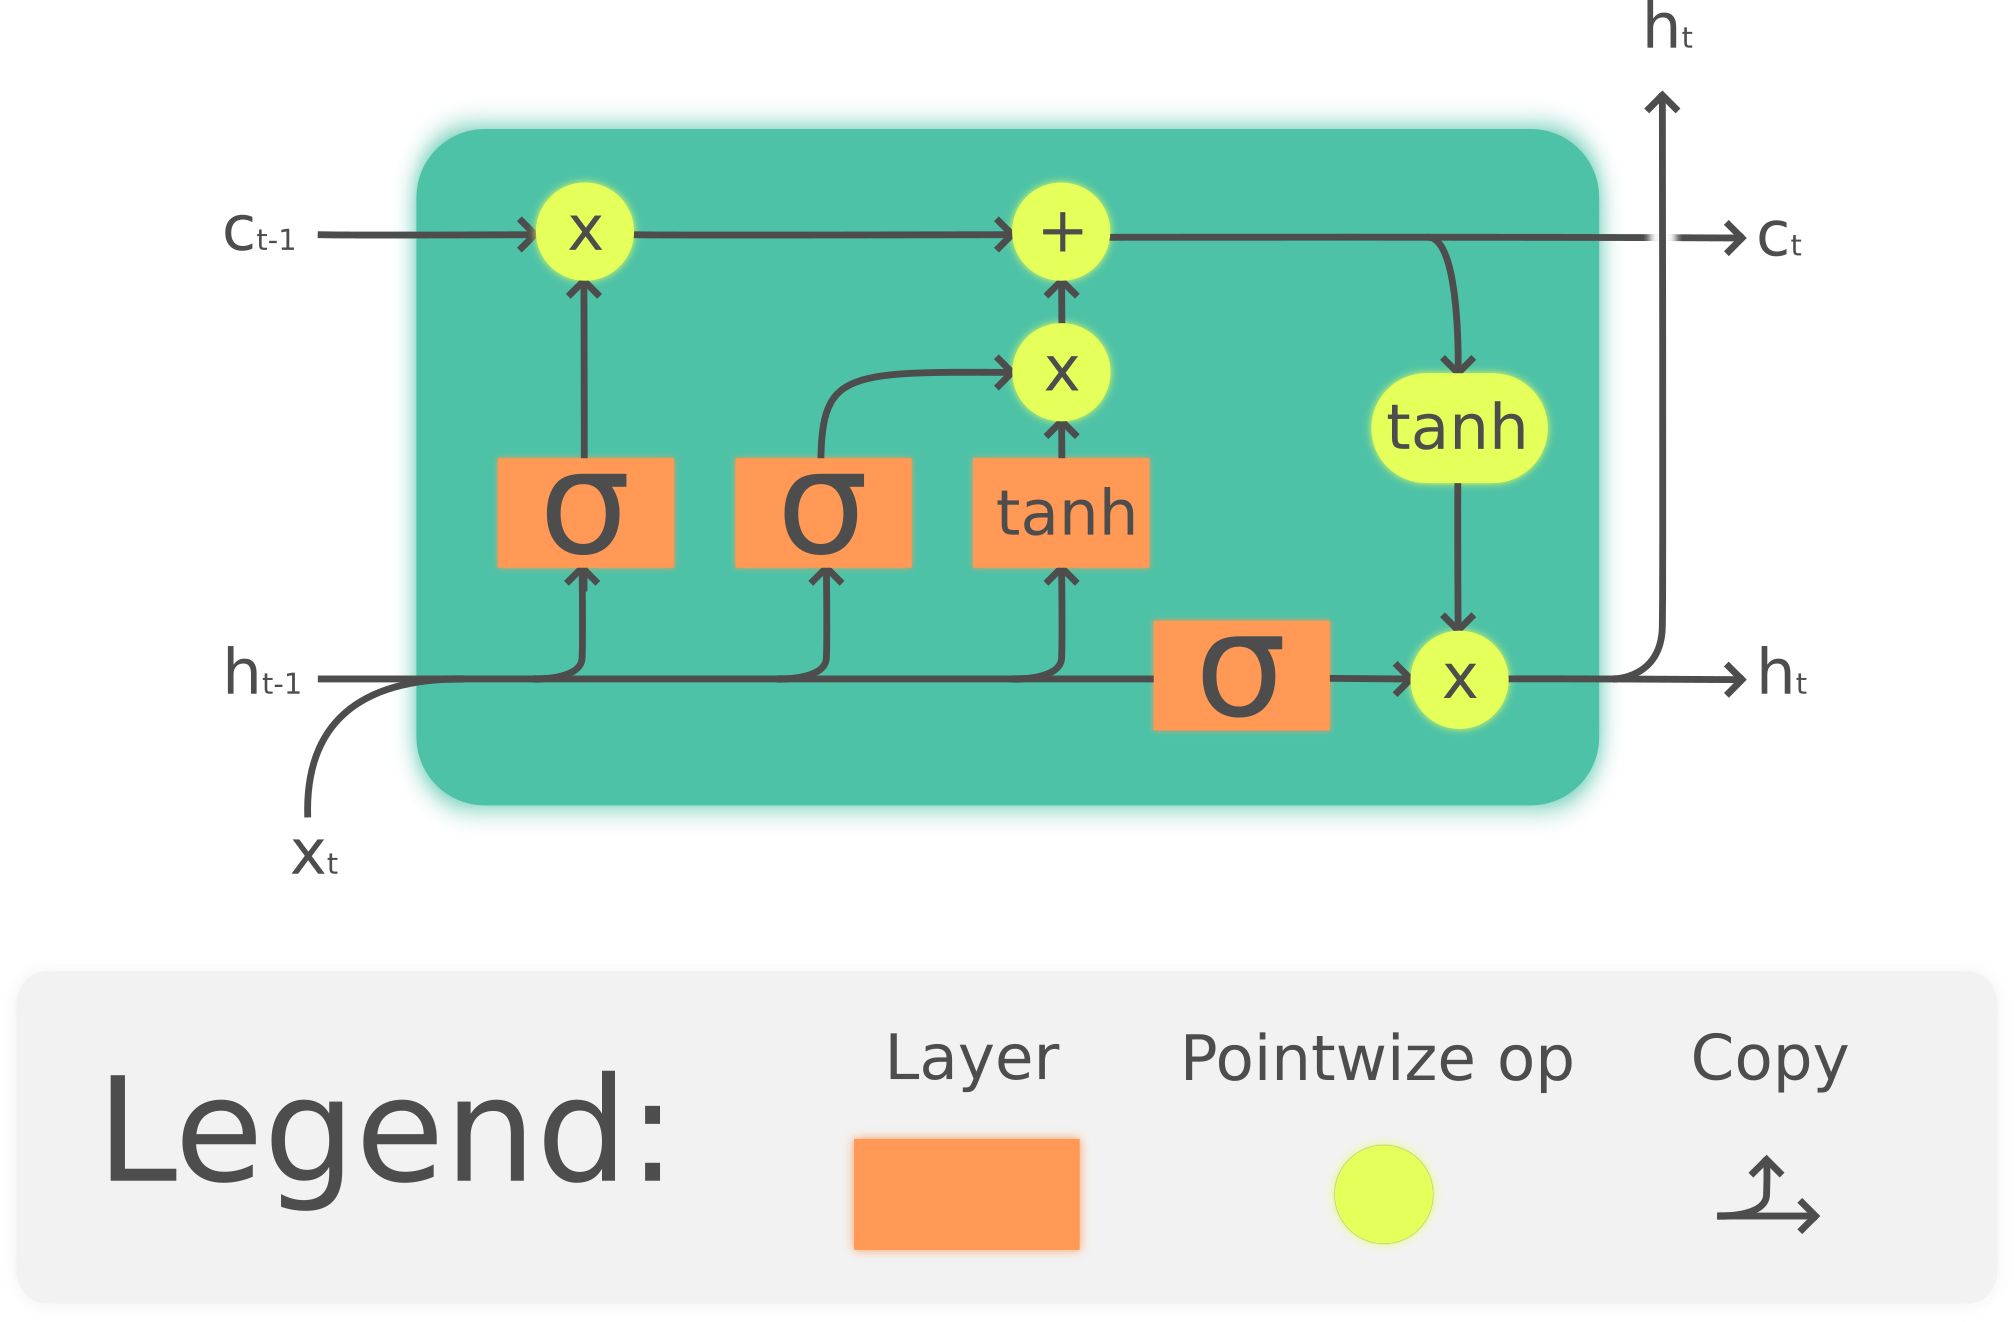
\includegraphics[width=12cm]{images/The_LSTM_cell.png}
\centering
\caption{The state cell of an LSTM model. (commons.wikimedia.org/wiki/File:The\_LSTM\_cell.png)}
\end{figure}

LSTMs have become the dominant model type in a variety of language tasks, including syntactic and morphological tasks. They significantly outperformed other types of models in SIGMORPHON 2016, since which time they have come to underlie nearly all morphology prediction models \parencite{Cotterell2016} \parencite{Cotterell2017}.

%% Basic algorithm template:
%\begin{algorithm}
%\caption{Algorithm Name}
%		\label{alg}
%		\begin{algorithmic}[1]
%			\Procedure{f}{}
%			\State $x$ = initialized variable
%			\For {i = 1 to n}
%	    	\State $x$ = $i$ + 1
%            \EndFor
%		    \State\Return $x$
%			\EndProcedure
%		\end{algorithmic}
%\end{algorithm}


